\documentclass[12pt]{article}
\usepackage[left=1cm, right=1cm, top=2cm,bottom=1.5cm]{geometry} 

\usepackage[parfill]{parskip}
\usepackage[utf8]{inputenc}
\usepackage[T2A]{fontenc}
\usepackage[russian]{babel}
\usepackage{enumitem}
\usepackage[normalem]{ulem}
\usepackage{amsfonts, amsmath, amsthm, amssymb, mathtools}
\usepackage{tabularx}
\usepackage{hhline}

\usepackage{accents}
\usepackage{fancyhdr}
\pagestyle{fancy}
\renewcommand{\headrulewidth}{1.5pt}
\renewcommand{\footrulewidth}{1pt}

\usepackage{graphicx}
\usepackage[figurename=Рис.]{caption}
\usepackage{subcaption}
\usepackage{float}

%%Наименование папки откуда забирать изображения
\graphicspath{ {./images/} }

%%Изменение формата для ввода доказательства
\renewcommand{\proofname}{$\square$  \nopunct}
\renewcommand\qedsymbol{$\blacksquare$}

%%Изменение отступа на таблицах
\addto\captionsrussian{%
	\renewcommand{\proofname}{$\square$ \nopunct}%
}
%% Римские цифры
\newcommand{\RN}[1]{%
	\textup{\uppercase\expandafter{\romannumeral#1}}%
}

%% Для удобства записи
\newcommand{\MR}{\mathbb{R}}
\newcommand{\MQ}{\mathbb{Q}}
\newcommand{\MN}{\mathbb{N}}
\newcommand{\MI}{\mathrm{I}}
\newcommand{\MJ}{\mathrm{J}}
\newcommand{\MH}{\mathrm{H}}
\newcommand{\MT}{\mathrm{T}}
\newcommand{\MU}{\mathcal{U}}
\newcommand{\MV}{\mathcal{V}}
\newcommand{\VN}{\varnothing}
\newcommand{\VE}{\varepsilon}

\theoremstyle{definition}
\newtheorem{defn}{Опр:}
\newtheorem{rem}{Rm:}
\newtheorem{prop}{Утв.}
\newtheorem{exrc}{Упр.}
\newtheorem{lemma}{Лемма}
\newtheorem{theorem}{Теорема}
\newtheorem{corollary}{Следствие}

\newenvironment{cusdefn}[1]
{\renewcommand\thedefn{#1}\defn}
{\enddefn}

\DeclareRobustCommand{\divby}{%
	\mathrel{\text{\vbox{\baselineskip.65ex\lineskiplimit0pt\hbox{.}\hbox{.}\hbox{.}}}}%
}
%Короткий минус
\DeclareMathSymbol{\SMN}{\mathbin}{AMSa}{"39}
%Длинная шапка
\newcommand{\overbar}[1]{\mkern 1.5mu\overline{\mkern-1.5mu#1\mkern-1.5mu}\mkern 1.5mu}
%Функция знака
\DeclareMathOperator{\sgn}{sgn}

%Обозначение константы
\DeclareMathOperator{\const}{\text{const}}

%Интеграл в большом формате
\DeclareMathOperator{\dint}{\displaystyle\int}

\newcommand{\smallerrel}[1]{\mathrel{\mathpalette\smallerrelaux{#1}}}
\newcommand{\smallerrelaux}[2]{\raisebox{.1ex}{\scalebox{.75}{$#1#2$}}}

\newcommand{\smallin}{\smallerrel{\in}}
\newcommand{\smallnotin}{\smallerrel{\notin}}

\newcommand*{\medcap}{\mathbin{\scalebox{1.25}{\ensuremath{\cap}}}}%
\newcommand*{\medcup}{\mathbin{\scalebox{1.25}{\ensuremath{\cup}}}}%

%Скалярное произведение
\DeclarePairedDelimiterX{\inner}[2]{\langle}{\rangle}{#1, #2}

%Подпись символов снизу
\newcommand{\ubar}[1]{\underaccent{\bar}{#1}}

\begin{document}
\lhead{Математический анализ - \RN{2}}
\chead{Шапошников С.В.}
\rhead{Лекция - 13}
\section*{Дифференцируемые отображения}
Пусть $X, Y$ - нормированные пространства, точка $a \in U \subset X$, функция $f\colon U \to Y$.
\begin{defn}
	Функция $f$ \uwave{дифференцируема} в точке $a$, если существует линейный непрерывный оператор $L$ и функция $\alpha \colon X \to Y$ такие, что:
	$$
	f(a + h) - f(a) = L(h) + \alpha(h){\cdot}\|h\|, \, \alpha(h) \colon \lim\limits_{h \to 0}{\alpha(h)} = 0
	$$ 
\end{defn}
\begin{defn}
	Линейный оператор $L$ из определения дифференцируемости $f$ называется \uwave{дифференциалом} $f$. Обозначается, как $df(a,h)$ или $df(h)$, если понимаем в какой точке все происходит.
\end{defn}
\begin{defn}
	Предел $\lim\limits_{t \to 0} \dfrac{f(a + tv) - f(a)}{t}$ называют \uwave{производной функции} $f$ \uwave{по вектору} $v$ и обозначают следующим образом: 
	$$
	\dfrac{\partial f}{\partial v}(a) = \lim\limits_{t \to 0} \dfrac{f(a + tv) - f(a)}{t}
	$$
\end{defn}
\begin{rem}
	Установили в прошлый раз, что если функция $f$ дифференцируема, то линейная часть $L(v)$ определяется следующим образом: $L(v) = \lim\limits_{t \to 0} \dfrac{f(a + tv) - f(a)}{t} = \dfrac{\partial f}{\partial v}(a)$ - производная по вектору $v$ и сказали, что $L(v) = df(a,v)$ - это дифференциал функции $v$.
\end{rem}

\section*{Частные случаи дифференцируемости функций}
\subsection*{$(\RN{1})$ Отображения из $\MR^n$ в $\MR$}

Пусть $f \colon \MR^n \to \MR$ дифференцируема в точке $a = (a_1, \dotsc, a_n)$. Если $f$ дифференцируема, то:
$$
	df(a,h) = \dfrac{\partial f}{\partial x_1}(a){\cdot}h_1 + \dotsc + \dfrac{\partial f}{\partial x_n}(a){\cdot} h_n
$$

\begin{defn}
	Производная вдоль вектора $e_k$: $\dfrac{\partial f}{\partial e_k}(a)$ называется \uwave{частной производной функции} $f$ \uwave{по переменной} $x_k$ \uwave{в точке $a$} и обозначается следующим образом: 
	$$
	\dfrac{\partial f}{\partial x_k}(a) = \dfrac{\partial f}{\partial e_k}(a) = \lim\limits_{t \to 0} \dfrac{f(a + te_k) - f(a)}{t}
	$$
\end{defn}
\begin{defn}
	Вектор состоящий из частных производных $\Big(\dfrac{\partial f}{\partial x_1}(a), \dotsc, \dfrac{\partial f}{\partial x_n}(a)\Big)$ в точке $a$ называется \uwave{градиентом функции} $f$ и обозначается следующим образом: 
	$$
	\text{grad}\, f(a) = \nabla f(a) = \Big(\dfrac{\partial f}{\partial x_1}(a), \dotsc, \dfrac{\partial f}{\partial x_n}(a)\Big)
	$$
\end{defn}

Поскольку дифференциал выражается через частные производные, то теперь несложно в некоторых случаях этот дифференциал найти.

\textbf{Пример}: $f(x_1,\dotsc,x_n) = x_k$ - линейная функция. У линейной функции дифференциал это она сама же. Чему будет равен $df(h)$? 
$$
	df(h) = \dfrac{\partial f}{\partial x_k}(a){\cdot}h_k = 1{\cdot}h_k = h_k = dx_k(h)
$$ 
Отметим, что $dx_1, \dotsc, dx_n$ - базис в сопряженном пространстве $(\MR^n)^*$. Дифференциал $df$ в точке $a$ по вектору приращения - линейная функция $\Rightarrow$ раскладывается по базисным линейным функциям. Либо мы просто заменяем $h_i$ на $dx_i(h)$. Используя полученный результат, мы можем переписать произвольный дифференциал в следующем виде:
$$
	df =  \dfrac{\partial f}{\partial x_1}dx_1 + \dotsc + \dfrac{\partial f}{\partial x_n}dx_n
$$
\begin{rem}
	Обычно могут объяснять, что $dx_i$ - малые приращения. Действительно, если подставить приращение $h$, то $dx_i$ даст компонент этого приращения. Но нельзя отождествлять функционал и его значение от вектора (вектор и ковектор).
\end{rem}

Дифференцирование не есть существование частных производных.

\textbf{Пример}: $f(x_1,x_2) = \begin{cases}
	0, & x_1 = 0 \vee x_2 = 0 \\
	1, & x_1 \neq 0 \wedge x_2 \neq 0
\end{cases}$;

У этой функции $f(x_1,0) \equiv 0 \Rightarrow \dfrac{\partial f}{\partial x_1}(0,0) = 0, \, f(0,x_2) \equiv 0 \Rightarrow\dfrac{\partial f}{\partial x_2}(0,0) = 0$. 
\begin{figure}[H]
	\centering
	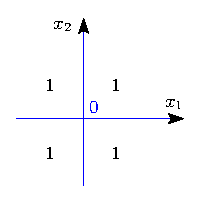
\includegraphics[width=0.2\textwidth]{13_1.eps}
	\caption{Пример недифференцируемой функции $f(x_1,x_2)$, имеющей частные производные.}
	\label{13_1}
\end{figure}
Но тем не менее $f$ не является дифференцируемой, поскольку она даже не является непрерывной в точке $(0,0)$.

Можно ли в терминах частных производных что-то говорить о дифференцируемости? Да, есть достаточное условие дифференцируемости в терминах частных производных.

\begin{theorem} \textbf{(Достаточное условие дифференцируемости)}
	Пусть $f \colon \MR^n \to \MR$ определена в окрестности точки $a$ и имеет в этой окрестности частные производные $\dfrac{\partial f}{\partial x_k}$, где $k = \overline{1,n}$. Если частные производные непрерывны в точке $a$, то $f$ дифференцируема в точке $a$.
\end{theorem}
\begin{proof}
	Докажем для случая $n=2$, оно ничем не будет отличаться от доказательства в общем, но будет нагляднее. Пусть $n = 2$.
	
	Рассмотрим приращение функции, вычтем и добавим слагаемое $f(a_1, a_2 + h_2)$:
	$$
		f(a_1 + h_1, a_2 + h_2) - f(a_1,a_2) = f(a_1 + h_1, a_2 + h_2) - f(a_1, a_2 + h_2) + f(a_1, a_2 + h_2) - f(a_1,a_2)
	$$	
	\begin{figure}[H]
		\centering
		\includegraphics[width=0.4\textwidth]{13_2.eps}
		\caption{Выбор $h_1, h_2$ в шаре, лежащем в $\MU$.}
		\label{13_2}
	\end{figure}
	Необходимо, чтобы функция $x_1 \mapsto f(x_1,a_2 + h_2)$ была непрерывной на отрезке и дифференцируемой на интервале. Тогда предположим, что на всём отрезке $[a_1, a_1+ h_1]$ эта функция дифференцируема: предположим, что $h = (h_1, h_2)$ достаточно мал так, что на отрезке $x_1 \in [a_1,a_1 + h_1]$ и $x_2 = a_2 + h_2$, а также на отрезке $x_2 \in [a_2, a_2 + h_2]$ и $x_1 = a_1$ в каждой точке существуют частные производные. Таким образом, на отрезках мы получим непрерывность и дифференцируемость.

	Используя теорему Лагранжа, применим её к функциям $x_1 \mapsto f(x_1,a_2 + h_2)$ и к $x_2 \mapsto f(a_1, x_2)$:
	$$
		f(a_1 + h_1, a_2 + h_2) - f(a_1, a_2 + h_2) + f(a_1, a_2 + h_2) - f(a_1,a_2) = \dfrac{\partial f}{\partial x_1}(c_1, a_2 + h_2){\cdot}h_1 + \dfrac{\partial f}{\partial x_2}(a_1, c_2){\cdot}h_2
	$$
	где $c_1$ лежит между $a_1$ и $a_1 + h_1$, а $c_2$ лежит между $a_2$ и $a_2 + h_2$. Тогда, если $h_1 \to 0$ и $h_2 \to 0$, то $c_1 \to a_1$ и $c_2 \to a_2$.
	$$
		\dfrac{\partial f}{\partial x_1}(c_1, a_2 + h_2){\cdot}h_1 + \dfrac{\partial f}{\partial x_2}(a_1, c_2){\cdot}h_2 = \dfrac{\partial f}{\partial x_1}(a_1, a_2 ){\cdot}h_1 + \dfrac{\partial f}{\partial x_2}(a_1, a_2){\cdot}h_2 +
	$$
	$$	
		+ \|h\|{\cdot}\bigg(\Big( \dfrac{\partial f}{\partial x_1}(c_1, a_2 + h_2) - \dfrac{\partial f}{\partial x_1}(a_1, a_2 ) \Big){\cdot}\dfrac{h_1}{\|h\|} + \Big( \dfrac{\partial f}{\partial x_2}(a_1, c_2) - \dfrac{\partial f}{\partial x_2}(a_1, a_2 ) \Big){\cdot}\dfrac{h_2}{\|h\|}\bigg)
	$$
	где $\|h\| = \sqrt{h_1^2 + h_2^2}$ и как следствие $\bigg|\dfrac{h_2}{\|h\|}\bigg| \leq 1, \, \bigg|\dfrac{h_2}{\|h\|}\bigg| \leq 1 \Rightarrow$ ограничены. Частные производные $f$ по условию непрерывны $\Rightarrow$ при $h_1 \to 0, h_2 \to 0$  получим $c_2 \to a_2$, $c_1 \to a_1$ и $a_2 + h_2 \to a_2$ тогда:
	$$
		\Big( \dfrac{\partial f}{\partial x_1}(c_1, a_2 + h_2) - \dfrac{\partial f}{\partial x_1}(a_1, a_2 ) \Big) \to 0, \, \Big( \dfrac{\partial f}{\partial x_2}(a_1, c_2) - \dfrac{\partial f}{\partial x_2}(a_1, a_2 ) \Big) \to 0	
	$$
	В итоге получаем:
	$$
		\|h\|{\cdot}\bigg(\Big( \dfrac{\partial f}{\partial x_1}(c_1, a_2 + h_2) - \dfrac{\partial f}{\partial x_1}(a_1, a_2 ) \Big){\cdot}\dfrac{h_1}{\|h\|} + \Big( \dfrac{\partial f}{\partial x_2}(a_1, c_2) - \dfrac{\partial f}{\partial x_2}(a_1, a_2 ) \Big){\cdot}\dfrac{h_2}{\|h\|}\bigg) = \|h\|{\cdot}\alpha(h), \, \lim\limits_{h \to 0} \alpha(h) = 0
	$$
	$$
		f(a_1 + h_1, a_2 + h_2) - f(a_1,a_2) = \dfrac{\partial f}{\partial x_1}(a_1, a_2 ){\cdot}h_1 + \dfrac{\partial f}{\partial x_2}(a_1, a_2){\cdot}h_2 + \alpha(h){\cdot}\|h\|, \, \lim\limits_{h \to 0} \alpha(h) = 0
	$$
\end{proof}
\subsection*{$(\RN{2})$ Отображения из $\MR^n$ в $\MR^m$}
Пусть $f \colon \MR^n \to \MR^m$. Функция $f$ устроена следующим образом: $f(x) = \begin{pmatrix}
	f_1(x) \\
	f_2(x) \\
	\vdots \\
	f_n(x)
\end{pmatrix}$. Если $f$ дифференцируема, то это значит, что каждая из компонент $f_i(x)$ дифференцируема или нет?
\begin{prop}
	Функция $f$ дифференцируема в точке $a \Leftrightarrow f_k$ дифференцируемы в точке $a$. Если $f$ дифференцируема в точке $a$, то $df(h) = J_f{\cdot}h$, где $J_f$ - матрица следующего вида:
	$$
		J_f = 
		\begin{pmatrix}
			\tfrac{\partial f_1}{\partial x_1} & \tfrac{\partial f_1}{\partial x_2} & \dotsc & \tfrac{\partial f_1}{\partial x_n} \\
			\tfrac{\partial f_2}{\partial x_1} & \tfrac{\partial f_2}{\partial x_2} & \dotsc & \tfrac{\partial f_2}{\partial x_n} \\
			\vdots & \vdots & \ddots & \vdots \\
			\tfrac{\partial f_m}{\partial x_1} & \tfrac{\partial f_m }{\partial x_2} & \dotsc & \tfrac{\partial f_m}{\partial x_n} 			
		\end{pmatrix} = 
		\begin{pmatrix}
			\nabla f_1 \\
			\nabla f_2 \\
			\vdots \\
			\nabla f_m
		\end{pmatrix}
	$$
\end{prop}
\begin{defn}
	Матрица $J_f$, определенная выше, называется \uwave{матрицей Якоби}.
\end{defn}
\begin{rem}
	Если $f$ дифференцируема, то при $x \approx a$ мы имеем $f(x) \approx f(a) + J_f{\cdot}(x-a)$ - аффинное отображение.
\end{rem}
\begin{proof}
	$f$ дифференцируема в точке $a \Leftrightarrow f(a+h) - f(a) = L(h) + \alpha(h)\|h\|, \, \lim\limits_{h \to 0} \alpha(h) = 0$. В векторной форме это запишется, как:
	$$
		\begin{pmatrix}
			f_1(a+h) - f_1(a)\\
			f_2(a+h) - f_2(a)\\
			\vdots\\
			f_m(a+h) - f_m(a)
		\end{pmatrix} = 
		\begin{pmatrix}
			L_1(h)\\
			L_2(h)\\
			\vdots\\
			L_m(h)
		\end{pmatrix} + 
		\begin{pmatrix}
			\alpha_1(h)\|h\|\\
			\alpha_2(h)\|h\|\\
			\vdots\\
			\alpha_m(h)\|h\|
		\end{pmatrix}
	$$
	что есть то же самое, что и следующее:
	$$
		\forall k = \overline{1,m},\, f_k(a+h) - f_k(a) = L_k(h) + \alpha_k(h)\|h\|, \, \lim\limits_{h \to 0} \alpha_k(h) = 0
	$$
	Поскольку каждая $f_k$ отображает $\MR^n \to \MR$, то мы знаем, что $L_k(h) = df_k(h) = \dfrac{\partial f_k}{\partial x_1}h_1 + \dotsc + \dfrac{\partial f_k}{\partial x_n}h_n$. Тем самым, мы получаем, что:
	$$
		L(h) = 	
		\begin{pmatrix}
			L_1(h)\\
			L_2(h)\\
			\vdots\\
			L_m(h)
		\end{pmatrix} = 
		\begin{pmatrix}
			\tfrac{\partial f_1}{\partial x_1} & \tfrac{\partial f_1}{\partial x_2} & \dotsc & \tfrac{\partial f_1}{\partial x_n} \\
			\tfrac{\partial f_2}{\partial x_1} & \tfrac{\partial f_2}{\partial x_2} & \dotsc & \tfrac{\partial f_2}{\partial x_n} \\
			\vdots & \vdots & \ddots & \vdots \\
			\tfrac{\partial f_m}{\partial x_1} & \tfrac{\partial f_m }{\partial x_2} & \dotsc & \tfrac{\partial f_m}{\partial x_n} 			
		\end{pmatrix}{\cdot}
		\begin{pmatrix}
			h_1\\
			h_2\\
			\vdots\\
			h_n
		\end{pmatrix} = 
		\begin{pmatrix}
			\nabla f_1 \\
			\nabla f_2 \\
			\vdots \\
			\nabla f_m
		\end{pmatrix}{\cdot}
		\begin{pmatrix}
			h_1\\
			h_2\\
			\vdots\\
			h_n
		\end{pmatrix}
	$$ 
\end{proof}

\newpage
\section*{Правила дифференцирования}
\begin{enumerate}[label ={(\arabic*)}]
	\item \textbf{Линейность}: Пусть $X,Y$ - нормированные пространства, $f,g \colon X \to Y$ - дифференцируемы в точке $a$. Тогда $\alpha f + \beta g$ - дифференцируема в точке $a$ и верно следующее: 
	$$
		d(\alpha f + \beta g) = \alpha {\cdot} df + \beta {\cdot} dg
	$$
	\begin{proof}
		По определению:
		$$
			\alpha f(a + h) + \beta g(a + h) - \alpha f(a) - \beta g(a) = \alpha (f(a+h) -f(a)) + \beta (g(a+h) - g(a)) = 
		$$
		$$
			= \alpha {\cdot} \big(df(h) + \gamma_1(h){\cdot}\|h\|\big) + \beta {\cdot} \big(dg(h) + \gamma_2(h){\cdot}\|h\|\big), \, \lim\limits_{h \to 0} \gamma_1(h) = 0, \, \lim\limits_{h \to 0} \gamma_2(h) = 0
		$$
		Раскроем скобки и получим линейную комбинацию линейных функций, то есть линейную функцию:
		$$
			\big(\alpha {\cdot} df(h) + \beta {\cdot} dg(h)\big) + \big(\alpha \gamma_1(h) + \beta \gamma_2(h) \big){\cdot} \|h\|, \, \lim\limits_{h \to 0} \big(\alpha \gamma_1(h) + \beta \gamma_2(h) \big) = 0
		$$
		где $\big(\alpha {\cdot} df(h) + \beta {\cdot} dg(h)\big)$ - линейная часть.
	\end{proof}
	\item \textbf{Правило Лейбница}: Пусть $X$ - нормированное пространство, $f,g \colon X \to \MR$ - дифференцируемы в точке $a$. Тогда $fg$ - дифференцируема в точке $a$ и верно следующее: 
	$$
		d(fg)(h) = f(a)dg(h) + g(a)df(h)
	$$
	\begin{proof}
		По определению дифференцируемости:
		$$
			f(a+h)g(a+h) - f(a)g(a) = \big(f(a + h) - f(a)\big){\cdot}g(a+h) + f(a){\cdot}\big(g(a+h) - g(a)\big) = 
		$$
		$$
			= \big(df(h) + \gamma_1(h)\|h\|\big){\cdot}\big(g(a) + \big(g(a+h) - g(a)\big)\big) + f(a){\cdot}\big(dg(h) + \gamma_2(h)\|h\|\big) = 
		$$
		$$
			= g(a){\cdot}df(h) + f(a){\cdot}dg(h) + \Big(g(a)\gamma_1(h) + \big(g(a+h) - g(a)\big)\big(\tfrac{df(h)}{\|h\|} + \gamma_1(h)\big) + f(a) \gamma_2(h) \Big){\cdot}\|h\|
		$$
		Получили линейную часть: $g(a)df(h) + f(a)dg(h)$. Поскольку $g$ - дифференцируема в точке $a \Rightarrow$ она непрерывна в этой точке, тогда:
		$$
			\lim\limits_{h \to 0} \big(g(a+h) - g(a)\big) = 0
		$$
		Рассмотрим оставшуюся часть, поскольку по определению $\forall i = 1,2, \, \lim\limits_{h \to 0} \gamma_i(h) = 0$, тогда:
		$$
			\lim\limits_{h \to 0} g(a) \gamma_1(h) = 0, \, \lim\limits_{h \to 0} f(a) \gamma_2(h) = 0, \, \lim\limits_{h \to 0} \big(g(a+h) - g(a)\big)\gamma_1(h) = 0
		$$
		
		По определению $df$ - непрерывный линейный оператор, следовательно $\|df(h)\| \leq C \|h\|$, тогда получим:
		$$
			\Big\|\big(g(a+h) - g(a)\big){\cdot}\tfrac{df(h)}{\|h\|}\Big\| = \Big|\big(g(a+h) - g(a)\big)\Big|{\cdot}\dfrac{1}{\|h\|}{\cdot}\|df(h)\| \leq C\Big|\big(g(a+h) - g(a)\big)\Big| \to 0
		$$
		То есть получили что-то стремящееся к нуля, умноженное на что-то ограниченное. Таким  образом остаточная часть выражения стремится к нулю при $h \to 0$:
		$$
			\lim\limits_{h\to 0}\Big(g(a)\gamma_1(h) + \big(g(a+h) - g(a)\big)\big(\tfrac{df(h)}{\|h\|} + \gamma_1(h)\big) + f(a) \gamma_2(h) \Big) = 0
		$$
	\end{proof}
	\newpage
	\item \textbf{Дифференцирование сложной функции}: Пусть $X, Y, Z$ - нормированные пространства, функция $f \colon X \to Y$ - дифференцируема в точке $a \in X$, $g\colon Y \to Z$ - дифференцируема в точке $f(a)$. Тогда $g(f(x))$ - дифференцируема в точке $a$ и верно следующее:
	$$
		dg(f) = dg(df)
	$$
	\begin{rem}
		$dg(f) = dg(df)$ это то же самое, что и $dg(f)(h) = dg\big(df(h)\big)$, а также $dg \circ f = dg \circ df$;
	\end{rem}
	\begin{proof}
		По определению:
		$$
			f(a+h) - f(a) = df(h) + \alpha(h)\|h\|,\, \lim\limits_{h \to 0} \alpha(h) = 0
		$$
		$$
			g\big(f(a)+v\big) - g\big(f(a)\big) = dg(v) + \beta(v)\|v\|,\, \lim\limits_{v \to 0} \beta(v) = 0
		$$
		Доопределим функцию $\beta$ в нуле: $\beta(0) = 0$, тогда $\beta$ - непрерывная в нуле функция. Подставим вместо $v$ разность $f(a+h) - f(a)$:
		$$
			g\big(f(a+h)\big) - g\big(f(a)\big) = dg\big(df(h) + \alpha(h)\|h\| \big) + \beta\big(df(h) + \alpha(h)\|h\| \big){\cdot}\big\|df(h) + \alpha(h)\|h\| \big\|
		$$
		Поскольку $dg(v)$ - линейный непрерывный оператор, то:
		$$
			dg\big(df(h) + \alpha(h)\|h\| \big) = dg\big(df(h)\big) + \|h\|{\cdot}dg\big(\alpha(h)\big)
		$$ 
		Так как, $dg$ непрерывна в нуле, то $\lim\limits_{h\to 0} dg\big(\alpha(h)\big) = 0$. Поскольку $\beta(v)$ непрерывна в нуле, то:
		$$
				\lim\limits_{h \to 0} \beta\big(df(h) + \alpha(h)\|h\| \big) = \lim\limits_{h \to 0} \beta\big(f(a+h) - f(a)\big) = 0
		$$
		Таким образом, получим:
		$$
			g\big(f(a+h)\big) - g\big(f(a)\big) =  dg\big(df(h)\big) + \|h\|{\cdot}\Big( dg\big(\alpha(h) \big) + \beta\big(f(a+h) - f(a)\big){\cdot}\Big\|\tfrac{df(h)}{\|h\|} + \alpha(h)\Big\| \Big) 
		$$
		По определению $df$ - непрерывный линейный оператор, следовательно $\|df(h)\| \leq C \|h\|$, тогда по неравенству треугольника:
		$$
			\Big\|\tfrac{df(h)}{\|h\|} + \alpha(h)\Big\| \leq \dfrac{\|df(h)\|}{\|h\|} + \|\alpha(h)\| \leq C + \|\alpha(h)\|
		$$
		Поскольку $\alpha(h)$ стремится к нулю, при $h \to 0$, то она ограничена, тогда получаем, что все выражение $\Big\|\tfrac{df(h)}{\|h\|} + \alpha(h)\Big\|$ - ограничено и умножается на что-то стремящееся к нулю, тогда:
		$$
			\lim\limits_{h \to 0} \Big( dg\big(\alpha(h) \big) + \beta\big(f(a+h) - f(a)\big){\cdot}\Big\|\tfrac{df(h)}{\|h\|} + \alpha(h)\Big\| \Big)  = 0
		$$
	\end{proof}
	\item \textbf{Дифференцирование обратной функции}: Пусть $X, Y$ - нормированные пространства, множества $\MU \subset X, \, \MV \subset Y$ - открытые. Если функция $f \colon \MU \to \MV$ - гомеоморфизм (биекция, отображение и обратное к нему - непрерывны), $f$ - дифференцируема в точке $a \in \MU$ и $df \colon X \to Y$ имеет  обратный оператор $(df)^{-1} \colon Y \to X$ - непрерывный линейный оператор. Тогда функция $f^{-1}\colon \MV \to \MU$ является дифференцируемой в точке $f(a)$ и верно следующее:
	$$
		df^{-1} = (df)^{-1}
	$$
	\begin{rem}
		Не вдаваясь в детали, требуем существование непрерывного обратного оператора.
	\end{rem}
	\begin{proof}
		Достаточно показать, что: 
		$$
			\lim\limits_{v \to 0} \dfrac{\|f^{-1}\big(f(a) + v\big) - f^{-1}\big(f(a)\big) - (df)^{-1}(v)\|}{\|v\|} = 0
		$$
		Сделаем замену: 
		$$
			v = f(a + h) - f(a), \, v \colon f(a) + v \in \MV, \, h \to 0 \Rightarrow v \to 0
		$$ 
		или же через $h$: 
		$$
			h = f^{-1}\big(f(a) + v\big) - a, \, v \to 0 \Rightarrow h \to 0
		$$ 
		что по сути является одним и тем же. Такая замена в пределе возможна поскольку по условию функция $f$ это гомеоморфизм $\Rightarrow$ биекция $\Rightarrow$ пока $h \neq 0$ такое $v$ не будет нулем $\Rightarrow$ можно применять теорему о пределе композиции функций (внутренняя функция не должна заходить в предельную точку). То есть берем  $v \neq 0 \Leftrightarrow h \neq 0$ и таким образом:
		$$
			\lim\limits_{v \to 0} \dfrac{\Big\|f^{-1}\big(f(a) + v\big) - f^{-1}\big(f(a)\big) - (df)^{-1}(v)\Big\|}{\|v\|} = \lim\limits_{h \to 0} \dfrac{\Big\|a + h - a - (df)^{-1}\big(df(h) + \alpha(h)\|h\|\big)\Big\|}{\Big\|df(h) + \alpha(h)\|h\|\Big\|} 
		$$
		Поскольку $(df)^{-1}$ - линейное отображение (обратное к линейному - линейно), то 
		$$
			h - (df)^{-1}\big(df(h) + \alpha(h)\|h\|\big) = h - (df)^{-1}\big(df(h)\big) -  (df)^{-1}\big(\alpha(h)\|h\|\big) = h - h - (df)^{-1}\big(\alpha(h)\big){\cdot}\|h\|
		$$
		и в итоге получим следующее:
		$$
			 \lim\limits_{h \to 0} \dfrac{\Big\|h - (df)^{-1}\big(df(h) + \alpha(h)\|h\|\big)\Big\|}{\Big\|df(h) + \alpha(h)\|h\|\Big\|} 
			 =  
			 \lim\limits_{h \to 0} \dfrac{\Big\| - (df)^{-1}\big(\alpha(h)\big){\cdot}\|h\|\Big\|}{\Big\|\tfrac{df(h)}{\|h\|} + \alpha(h)\Big\|{\cdot}\|h\|} 
			 = 
			 \lim\limits_{h \to 0} \dfrac{\Big\|- (df)^{-1}\big(\alpha(h)\big)\Big\|}{\Big\|\tfrac{df(h)}{\|h\|} + \alpha(h)\Big\|} 
		$$
		Поскольку $(df)^{-1}$ - линейный непрерывный оператор, то $\|(df)^{-1}(y)\| \leq C^{-1} \|y\|$, подставим $y = df(h)$ и получим $\|h\| \leq C^{-1} \|df(h)\|$, тогда по неравенству треугольника:
		$$
			\Big\|\tfrac{df(h)}{\|h\|} + \alpha(h)\Big\| \geq \dfrac{\|df(h)\|}{\|h\|} - \|-\alpha(h)\| = \dfrac{\|df(h)\|}{\|h\|} - |-1|{\cdot}\|\alpha(h)\| = \dfrac{\|df(h)\|}{\|h\|} - \|\alpha(h)\|\geq C - \|\alpha(h)\|
		$$
		Таким образом, при достаточно малых $h$, знаменатель будет больше, чем $C - \|\alpha(h)\| \geq \tfrac{C}{2}$, поскольку при малых $h$ верно $\|\alpha(h)\| \approx 0$ по определению. Тогда:
		$$
			0 \leq \dfrac{\Big\|-(df)^{-1}\big(\alpha(h)\big)\Big\|}{\Big\|\tfrac{df(h)}{\|h\|} + \alpha(h)\Big\|} \leq - \tfrac{2}{C}\Big\|(df)^{-1}\big(\alpha(h)\big)\Big\| \xrightarrow[h \to 0]{} 0 \Rightarrow \lim\limits_{h \to 0} \dfrac{\Big\|- (df)^{-1}\big(\alpha(h)\big)\Big\|}{\Big\|\tfrac{df(h)}{\|h\|} + \alpha(h)\Big\|}  = 0
		$$
	\end{proof}
\end{enumerate}

\begin{rem}
	Заметим, что формулировки и доказательства для нормированных пространств повторяют те же самые формулировки и доказательства в одномерном случае. И таким образом, сложность для понимания будет заключаться в том, чтобы перейти от нормированных пространств к $\MR^n$.
\end{rem}
\begin{rem}
	В одномерном случае утверждение о том, что можно продифференцировать обратную функцию состоит в том, что $f^\prime \neq 0$. Аналогом этого здесь является обратимость дифференциала.
\end{rem}

\end{document}